\textbf{Ejemplo 11}

Una persona se comprometió a pagar 250.000 COP en 3 meses, 300.000 COP en 8 meses y 130.000 COP en 15 meses. Ante la dificultad de cumplir con las obligaciones tal como están pactadas solicita una nueva forma de pago así: 60.000 COP hoy, 500.000 COP en 12 meses y el saldo en 18 meses. Suponiendo que la tasa de interés de oportunidad es del 36 \% nominal anual mes vencido, determinar el valor del saldo.
\\

\begin{table}
  \centering
  \resizebox{\columnwidth}{!}{%
  \begin{tabular}{|cll|}
  \hline
  \multicolumn{3}{|c|}{\cellcolor[HTML]{FFB183}\textbf{1. Asignación período focal}}  \\ \hline
  \multicolumn{3}{|c|}{pf = 8pmv}                                                     \\ \hline
  \multicolumn{3}{|c|}{\cellcolor[HTML]{FFB183}\textbf{2. Declaración de variables}}  \\ \hline
  \multicolumn{3}{|c|}{\cellcolor[HTML]{FFB183}\textbf{2.1 Deuda inicial}}            \\ \hline
  \multicolumn{1}{|l|}{\begin{tabular}[c]{@{}l@{}}$P_1 = 250.000$ COP\\ $n_1 = 5pmv$\end{tabular}} &
    \multicolumn{1}{l|}{\begin{tabular}[c]{@{}l@{}}$P_2 = 300.000$ COP\\ $n_2 = 0 pmv$\end{tabular}} &
    \begin{tabular}[c]{@{}l@{}}$F_3 = 130.000$ COP\\ $n_3 = -7pmv$\end{tabular} \\ \hline
  \multicolumn{3}{|c|}{$j = 36\%$ namv $\equiv i = 3\%$ pmv}                               \\ \hline
  \multicolumn{3}{|c|}{\cellcolor[HTML]{FFB183}\textbf{2.2 Deuda equivalente}}        \\ \hline
  \multicolumn{1}{|l|}{\begin{tabular}[c]{@{}l@{}}$P_4 = 60.000$ COP\\ $n_4 = 8$ pmv\end{tabular}} &
    \multicolumn{1}{l|}{\begin{tabular}[c]{@{}l@{}}$F_5 = 500.000$ COP\\ $n_5 = -4$ pmv\end{tabular}} &
    \begin{tabular}[c]{@{}l@{}}$F_6 = ?$ COP\\ $n_6 = −10$ pmv\end{tabular} \\ \hline
  \multicolumn{3}{|c|}{$j = 36\%$ namv $ \equiv i = 3\%$ pmv}                               \\ \hline
  \multicolumn{3}{|c|}{\cellcolor[HTML]{FFB183}\textbf{3. Diagrama de flujo de caja}} \\ \hline
  \multicolumn{3}{|c|}{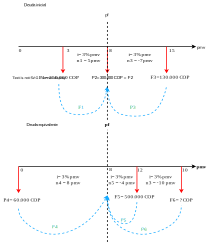
\includegraphics[trim=-5 -5 -5 -5 , scale=0.8]{2_Capitulo/img/ejemplos/11/Ejemplo 11ver.pdf} } \\ \hline
  \multicolumn{3}{|c|}{\cellcolor[HTML]{FFB183}\textbf{4. Declaración de fórmulas}}   \\ \hline
  \multicolumn{3}{|l|}{\begin{tabular}[c]{@{}l@{}}
    $F_1 + P_2 + P_3 = F_4 + P_5 + P_6$ Ecuación de equivalencia\\ 
    $F = P(1+i)^n$ Valor futuro\\ 
    $P = F(1 + i)^{−n}$ Valor presente (en pf)\end{tabular}} \\ \hline
  \multicolumn{3}{|c|}{\cellcolor[HTML]{FFB183}\textbf{5. Desarrollo matemático}}     \\ \hline
  \multicolumn{3}{|c|}{$250.000 $ COP $ (1+0.03)^{5}$$+ 300.000$ COP $(1+0.03)^0$$+ 130.000$ COP $(1+0.03)^{-7}$} \\
  \multicolumn{3}{|c|}{$=$} \\
  \multicolumn{3}{|c|}{$60.000$ COP $(1+0.03)^{8}$$+ 500.000$ COP $(1+0.03)^{-4}$$+ F_6$ COP $(1+0.03)^{-10}$} \\ \hline
  \multicolumn{3}{|c|}{\cellcolor[HTML]{FFB183}\textbf{6. Respuesta}}                 \\ \hline
  \multicolumn{3}{|c|}{
  {$F_6$ =235.549,16 COP Valor del saldo}}                            \\ \hline
  \end{tabular}%
  }
\end{table}
\pagebreak
